%!TEX TS-program = xelatex
%!TEX encoding = UTF-8 Unicode

% Modify the following line to match your school
% Available options include `Harvard`, `Princeton`, and `NYU`.
\documentclass[School=Harvard]{Dissertate}

\usepackage{pdfpages}

\usepackage{color}
\definecolor{bluekeywords}{rgb}{0.13,0.13,1}
\definecolor{greencomments}{rgb}{0,0.5,0}
\definecolor{redstrings}{rgb}{0.9,0,0}
\definecolor{grey}{rgb}{0.5,0.5,0.5}

\usepackage{listings}
\lstset{
    basicstyle=\scriptsize\ttfamily,
    breakatwhitespace=false,
    breaklines=false,
    commentstyle=\color{greencomments},
    escapeinside={(*@}{@*)},
    keywordstyle=\color{bluekeywords}\bfseries,
    language=Python,
    numbers=left,
    numbersep=5pt,
    numberstyle=\tiny\color{grey},
    showspaces=false,
    showstringspaces=false,
    showtabs=false,
    stringstyle=\color{redstrings}
}

\begin{document}

\frontmatter
\pagenumbering{roman}
% Some details about the dissertation.
\title{How to cook an egg}
\author{Josiah Wolf Oberholtzer}
\advisor{Hans Tutschku \& Chaya Czernowin}

% ... about the degree.
\degree{Doctor of Philosophy}
\field{Music Composition}
\degreeyear{2015}
\degreemonth{May}
\department{Music}

% ... about the candidate's previous degrees.
\pdOneName{B.Mus.}
\pdOneSchool{Oberlin Conservatory}
\pdOneYear{2006}

%\pdTwoName{M.A.}
%\pdTwoSchool{Monster's Univeristy}
%\pdTwoYear{2021}
\maketitle
\copyrightpage
\abstractpage
\tableofcontents
%\listoffigures
\dedicationpage
\acknowledgments

\mainmatter
\doublespacing
\cleardoublepage
\pagenumbering{arabic}
\setcounter{page}{1}
\setcounter{chapter}{-1}

\chapter{Introduction}

foo

\chapter{Mise-en-place}

\section{LilyPond}

\section{Python}

\section{Abjad}

\section{Consort}

\chapter{\emph{Abjad}: a musical model}

\section{Components: leaves \& containers}

\section{Durations, offsets and timespans}

\section{Indicators: context scope and annotations}

\section{Spanners}

\section{Selections and selectors}

\section{LilyPond format bundles}

\section{Agents}

\chapter{\emph{Consort}: A theory of composition}

foo

\chapter{\emph{Consort}: a theory of composition}

\chapter{Laying out time}

foo

\chapter{Laying out time}

foo

\chapter{Handlers}

foo

\chapter{\emph{Aurora} (2011)}

\cleardoublepage

\includepdf[pages=-]{scores/aurora-score.pdf}

\chapter{\emph{Plague Water} (2014)}

foo

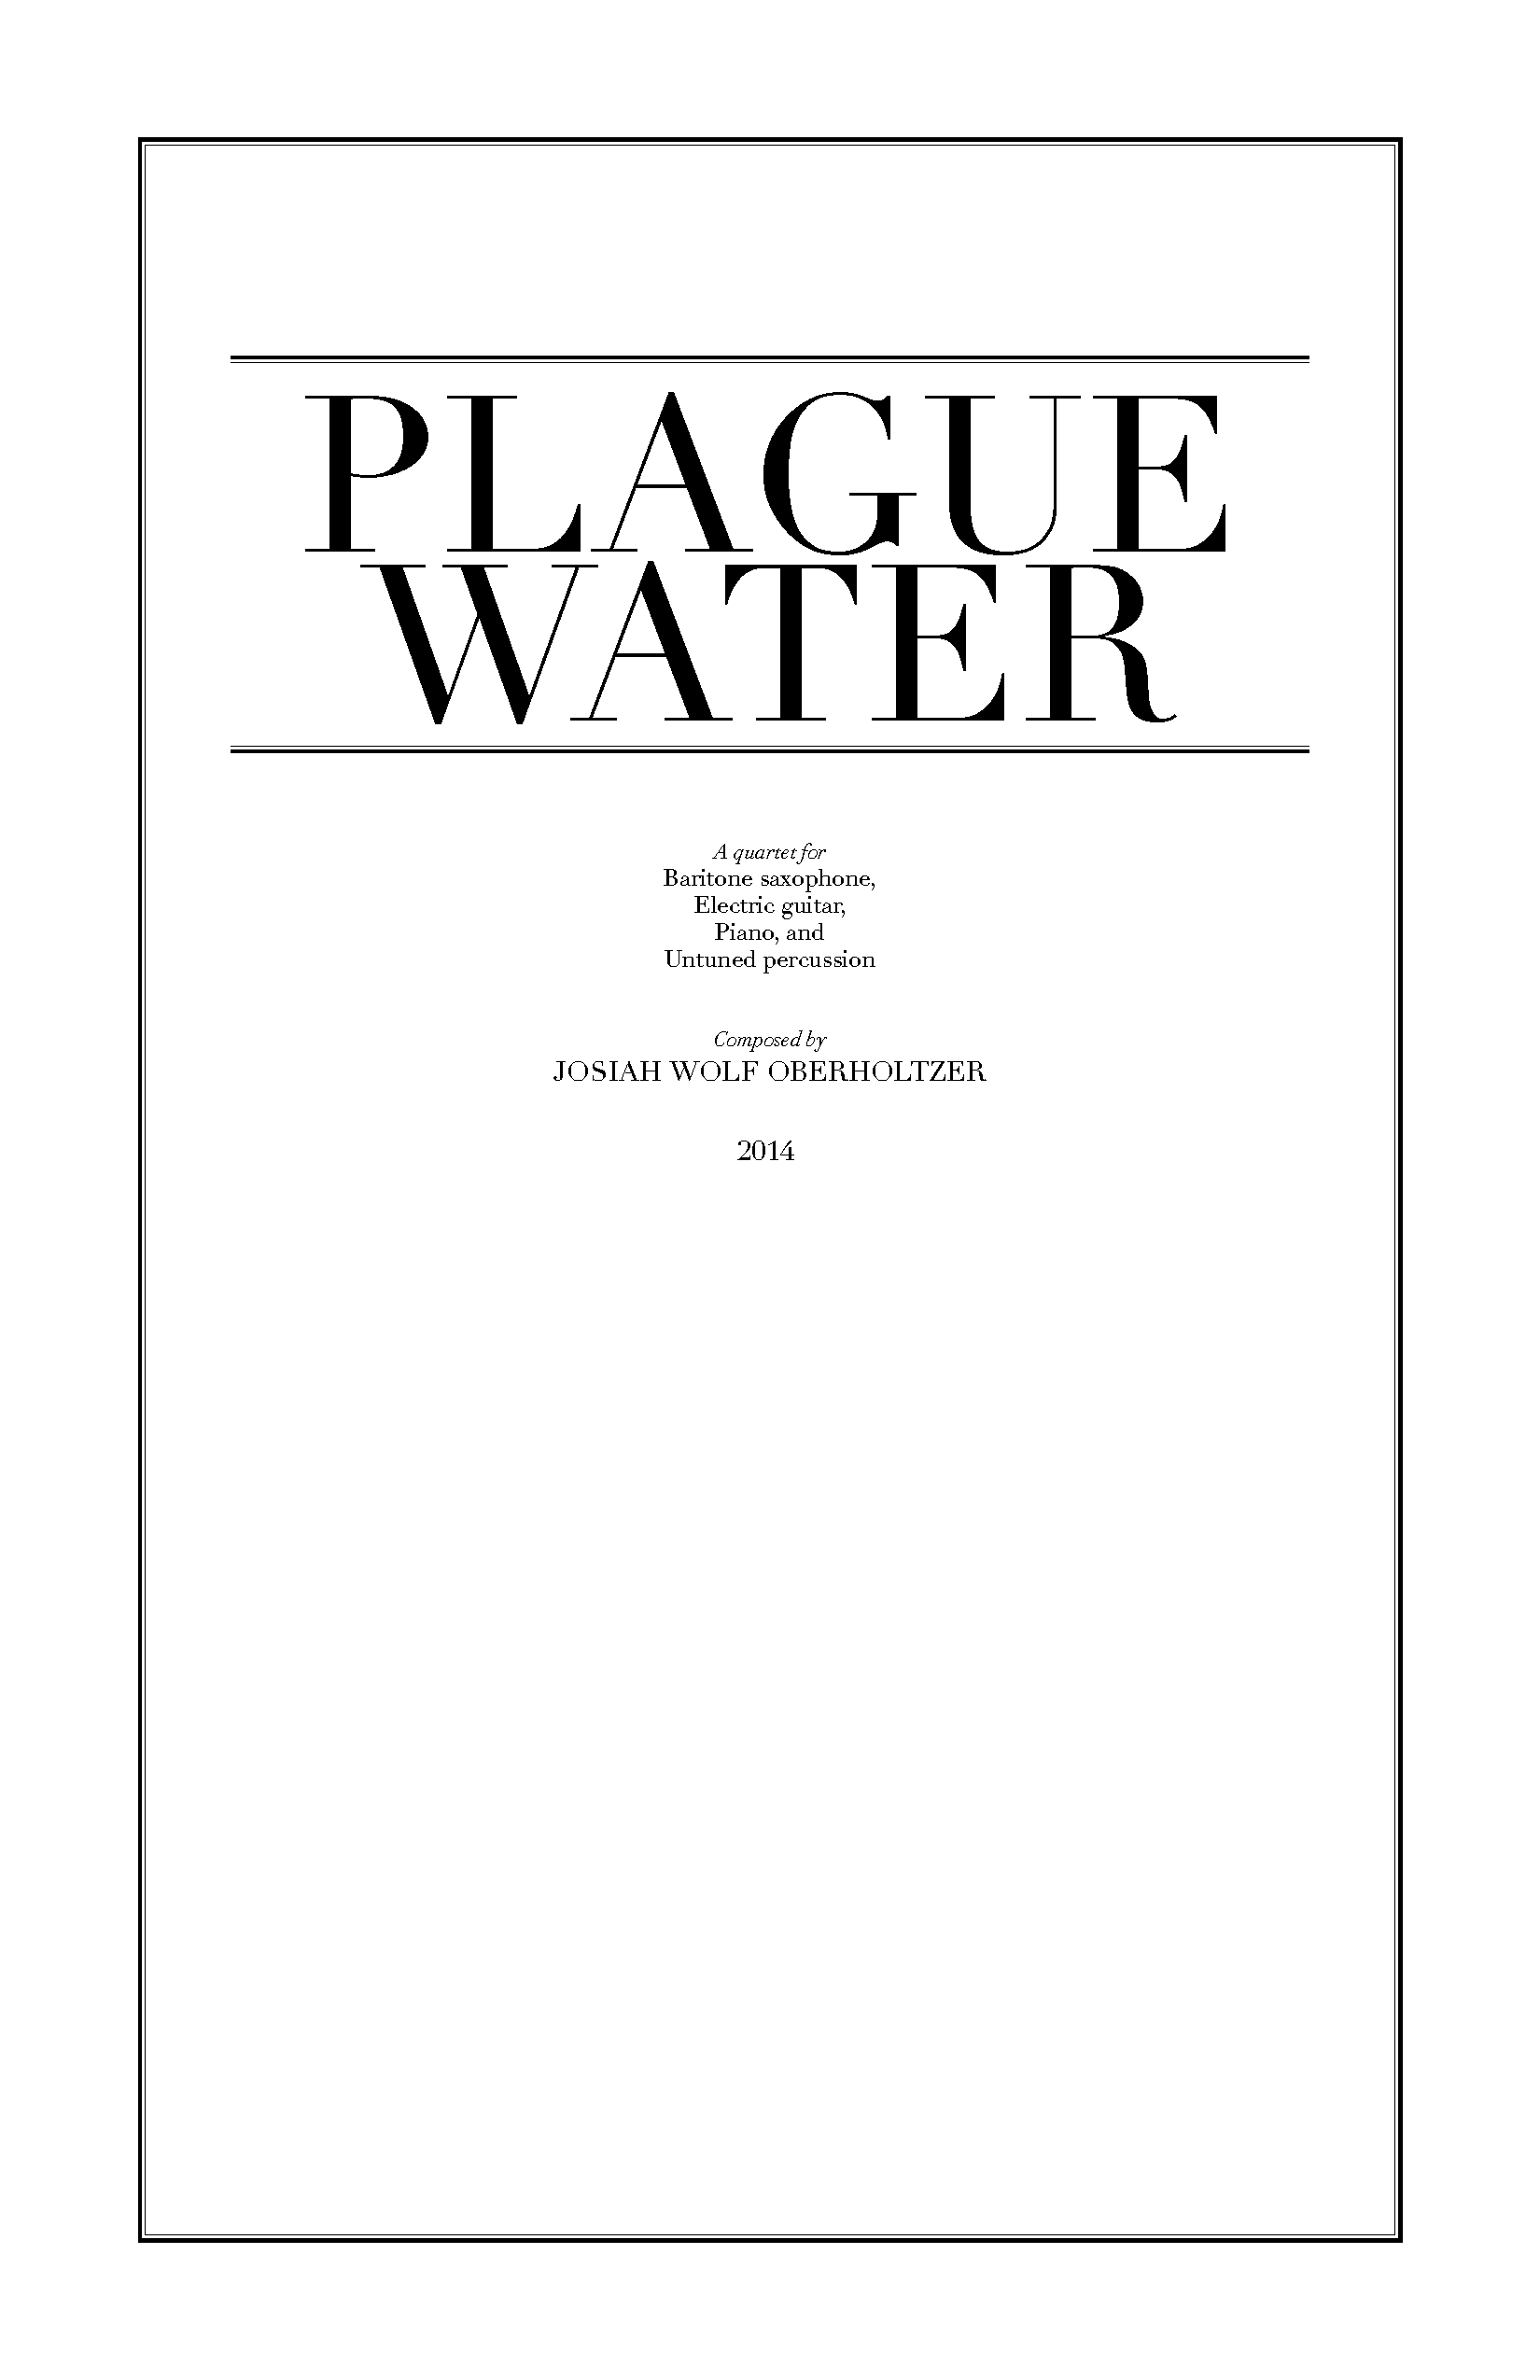
\includepdf[pages=-]{scores/plague-water-score.pdf}

\chapter{Invisible Cities (i): Zaira}

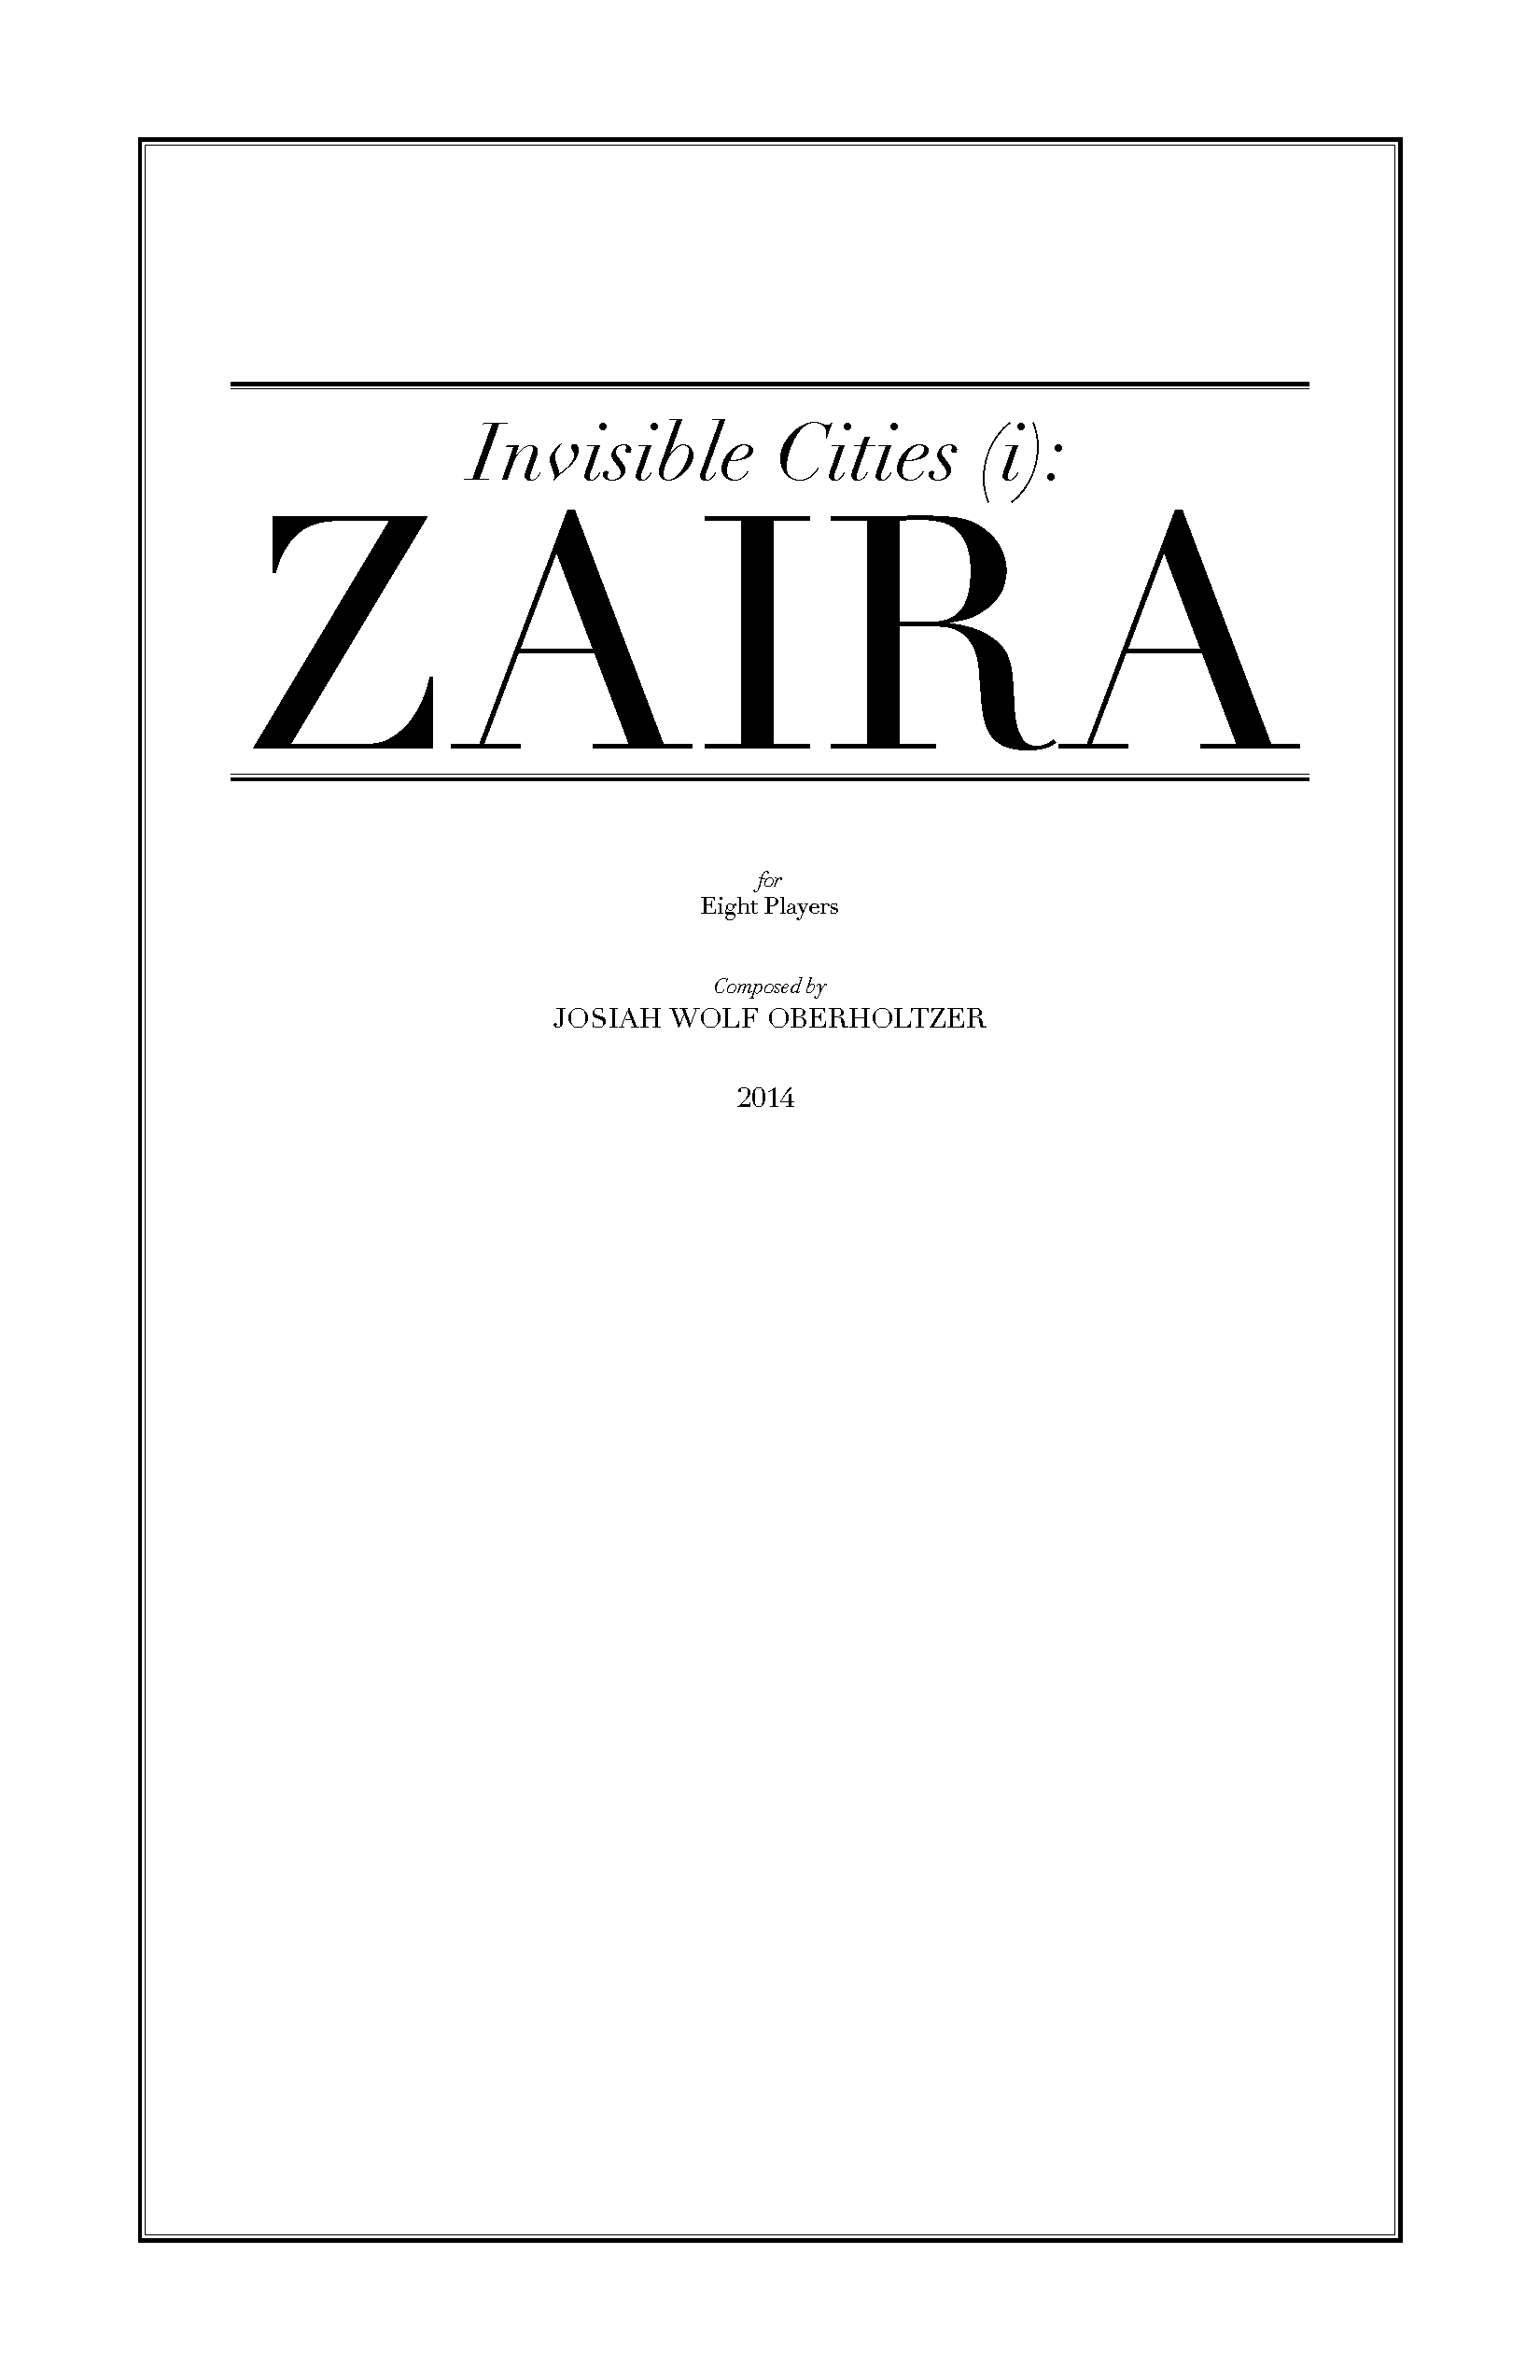
\includepdf[pages=-]{scores/zaira-score.pdf}

\chapter{Invisible Cities (ii): Armilla}

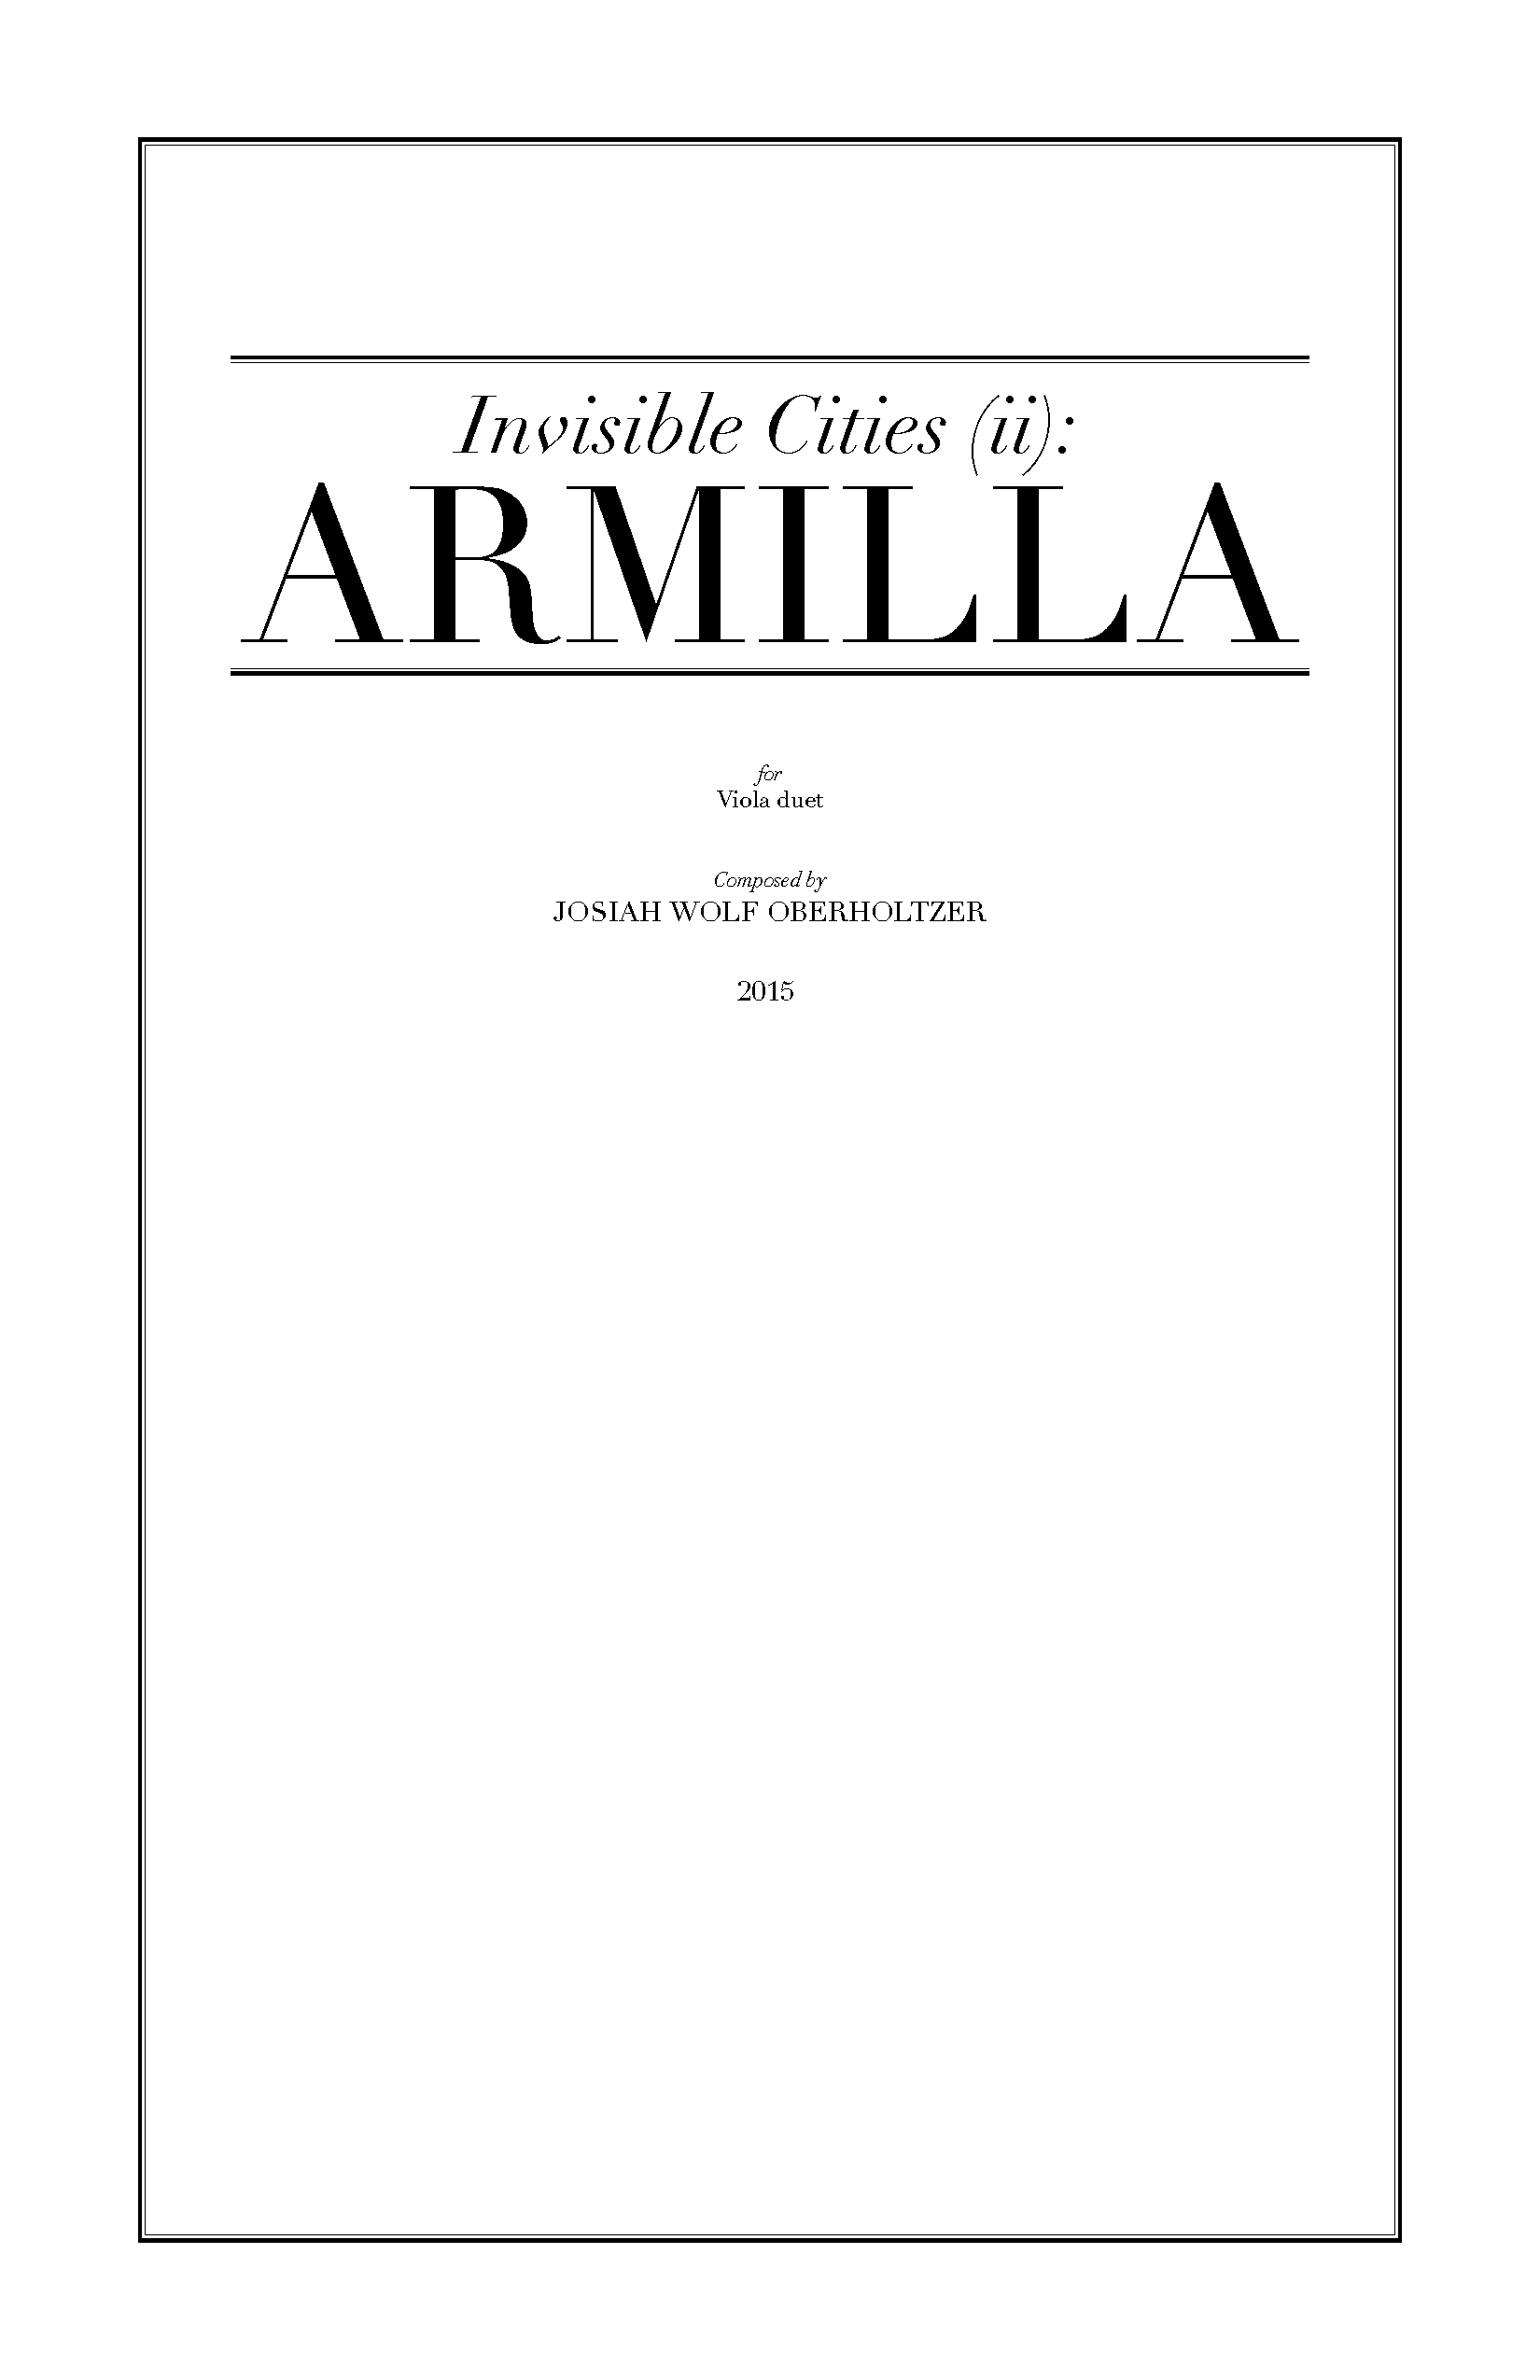
\includepdf[pages=-]{scores/armilla-score.pdf}

\chapter{\emph{Invisible Cities (iii): Ersilia} (2015)}

\cleardoublepage

%\includepdf[pages=-]{scores/ersilia-score.pdf}

\chapter{Conclusion}

foo

\begin{appendices}
    \section{Appendices}

\input{consort/index.tex}

\input{zaira/index.tex}

\input{armilla/index.tex}
\end{appendices}

\singlespacing

% the back matter
\clearpage
\bibliography{references}
\addcontentsline{toc}{chapter}{References}
\bibliographystyle{apalike2}

\newpage

% If you do want an image in the colophon:
\begin{figure}
    \vspace{50pt}
    \centering
    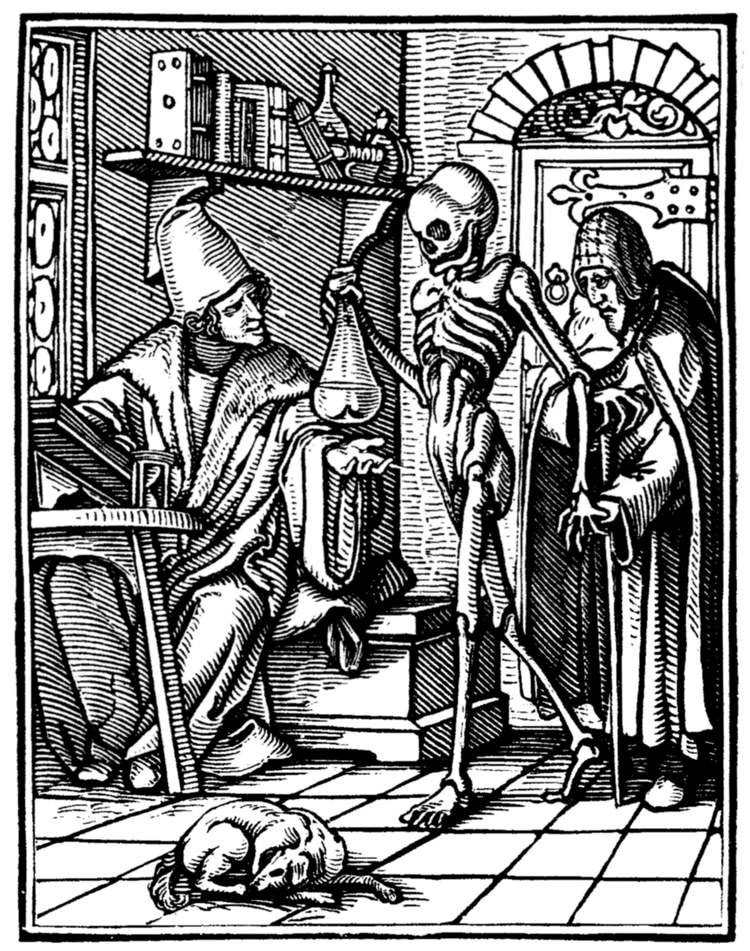
\includegraphics[width=0.51\textwidth]{endmatter/holbein-physician.jpg}
    \\
    \emph{The Physician}
    \\
    from Hans Holbein's \emph{Danse Macabre}
\end{figure}

% If you don't want an image in the colophon:
% \vspace*{200pt}

\begin{center}
\parbox{200pt}{\lettrine[lines=3,slope=-2pt,nindent=-4pt]{\textcolor{SchoolColor}{T}}{his
thesis was typeset} using \LaTeX, originally developed by Leslie Lamport and
based on Donald Knuth's \TeX. The body text is set in 11 point Egenolff-Berner
Garamond, a revival of Claude Garamont's humanist typeface. }
\end{center}

\end{document}